\documentclass[11pt]{article}

\usepackage[margin=1in]{geometry}
\usepackage{booktabs}
\usepackage{graphicx}
\usepackage{hyperref}

\title{Supplementary Diagnostics for Robust Low-Thrust Cislunar Maneuver Initialization Under Missed-Thrust Events}
\author{Anonymous Author}
\date{}

\begin{document}
\maketitle

\section*{Purpose}

This supplement preserves figure-only diagnostics that are secondary to the main manuscript's claim hierarchy. The main paper reports the tables, statistics, and claim-to-artifact map; the figures here support visual inspection of selected diagnostics without changing the recorded data values.

\section*{Teacher-Controlled Diagnostics}

\begin{figure}[h]
\centering
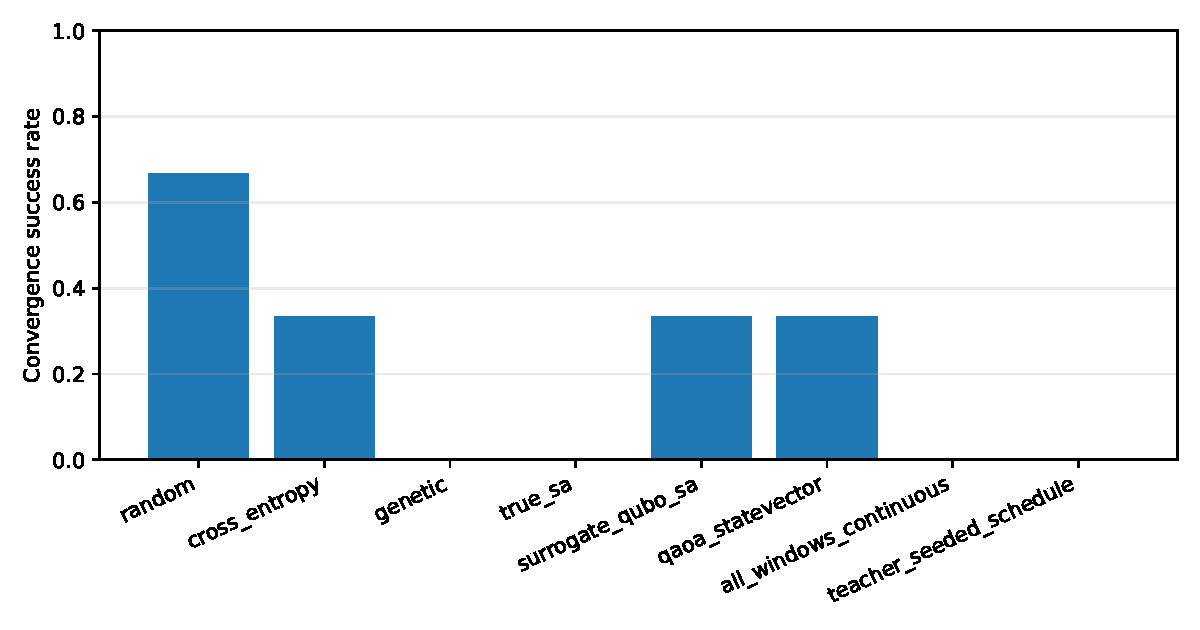
\includegraphics[width=0.78\linewidth]{../figures/teacher_feasible/refinement_success.pdf}
\caption{Teacher-controlled selected-branch refinement success rates. The result demonstrates nonzero recovery success but not quantum advantage.}
\label{fig:supp_teacher_success}
\end{figure}

\begin{figure}[h]
\centering
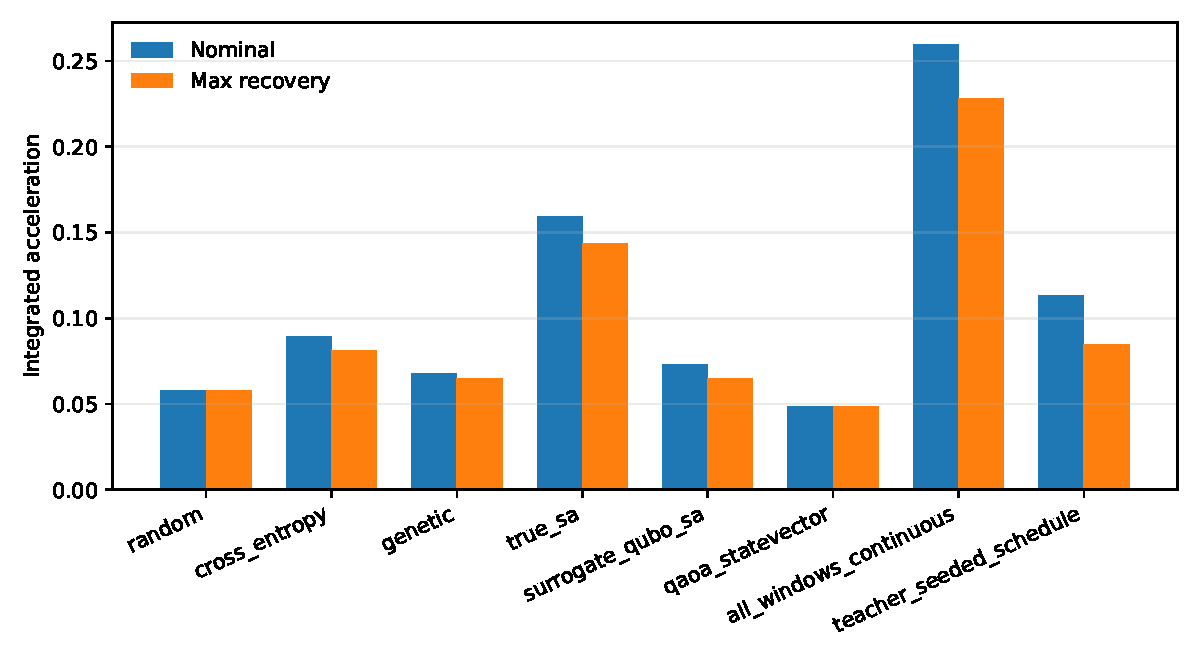
\includegraphics[width=0.78\linewidth]{../figures/teacher_feasible/recovery_fuel.pdf}
\caption{Teacher-controlled nominal and recovery fuel summaries. Fuel differences must be interpreted together with feasibility and missed-thrust error.}
\label{fig:supp_teacher_fuel}
\end{figure}

\begin{figure}[h]
\centering
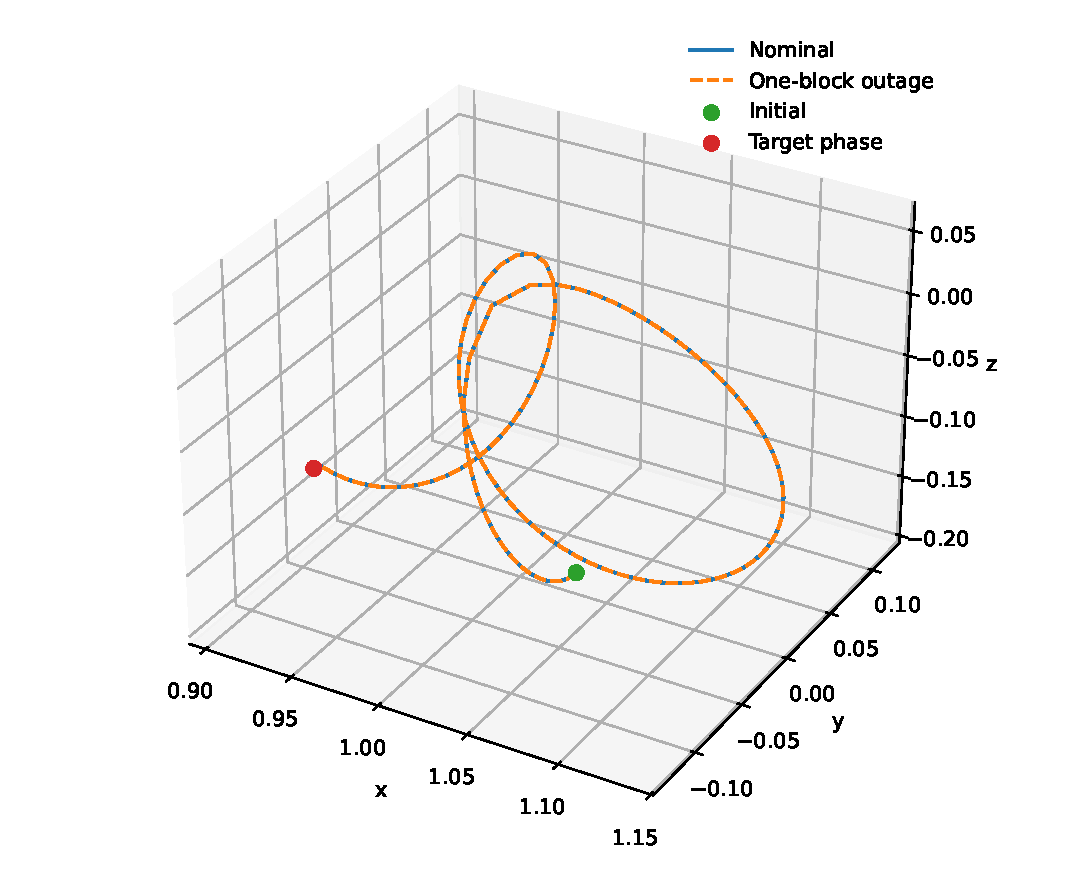
\includegraphics[width=0.78\linewidth]{../figures/teacher_feasible/trajectory_example.pdf}
\caption{Example trajectory from the teacher-controlled benchmark. The case is a normalized CR3BP algorithm benchmark, not a flight-ready trajectory.}
\label{fig:supp_teacher_traj}
\end{figure}

\section*{Catalog-Derived Feasibility Diagnostic}

\begin{figure}[h]
\centering
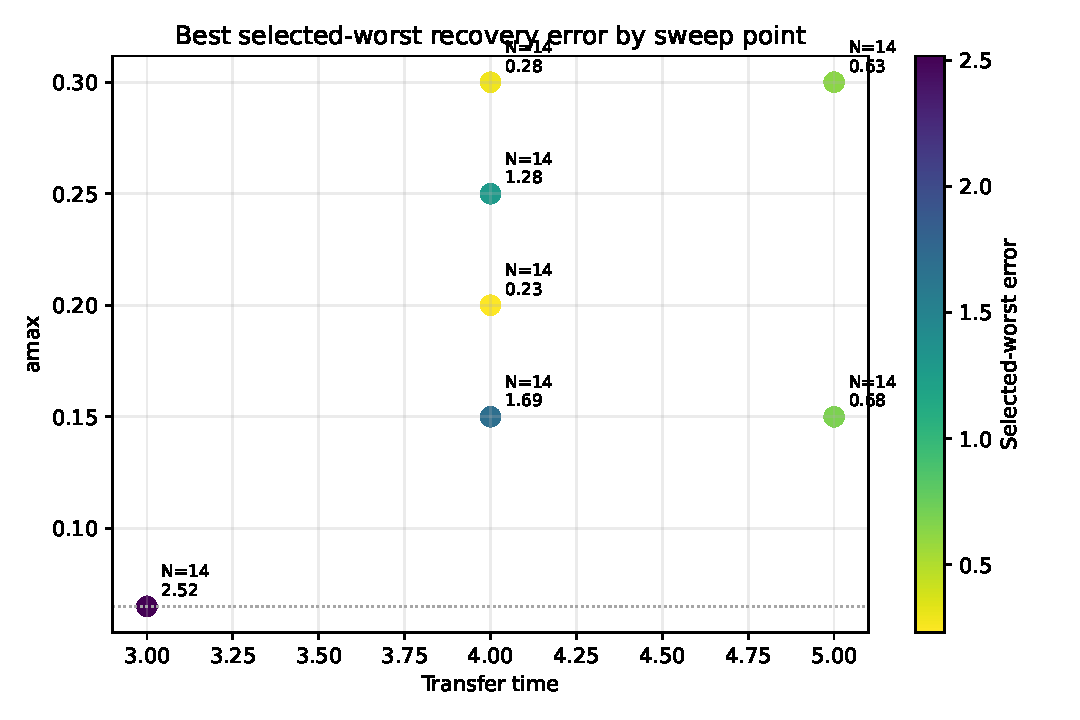
\includegraphics[width=0.78\linewidth]{../figures/feasibility_heatmap.pdf}
\caption{Feasibility sweep heatmap for the catalog-derived benchmark. The completed cases remain outside the configured robust success thresholds.}
\label{fig:supp_feasibility}
\end{figure}

\section*{Artifact Pointer}

The machine-readable manifest \path{../data/results/artifact_manifest.json} records hashes for the manuscript, supplement, source code, generated tables, figures, and result artifacts. It excludes itself, virtual environments, caches, logs, and LaTeX auxiliary files.

\end{document}
